\documentclass[UTF8, letterpaper, 14pt]{article}
\usepackage{geometry}
\geometry{left=3cm,right=3cm,top=3cm,bottom=3cm}
\usepackage{listings}
\usepackage{hyperref}
\usepackage{amsmath}
\usepackage{algorithm}
\usepackage{algorithmicx}
\usepackage{algpseudocode}
\usepackage{mathtools}
\DeclarePairedDelimiter\ceil{\lceil}{\rceil}
\DeclarePairedDelimiter\floor{\lfloor}{\rfloor}
\usepackage{graphicx}
\graphicspath{ {images/} }
\linespread{1.25}
\usepackage{tikz, mathpazo}
\usetikzlibrary{shapes.geometric, arrows}
\usepackage{setspace}

\begin{document}
\title{JPEG Family: Near-Lossless Compression Method Comparsion Study}
\author{Pengzhan Hao \\ \href{mailto:phao3@binghamton.edu}{phao3@binghamton.edu}}
\date{\today}
\maketitle
\begin{abstract}
The Joint Photographic Experts Group (JPEG) is a well-known committee which owns lots of image standards. Popluar lossy image compression standard JPEG is first work of them. After JPEG format became more popluar, JPEG committee released serveral new image compression method and corresponding image format, including JPEG2000, JPEG-LS, JPEG XT and etc. In my course project, I will concentrate two mainly used format, JPEG2000 and JPEG-LS, throughly state their technolgies and algorithms. Briefly introducation of my implemetation and comparsion these two algorithms and JPEG will be also covered in this report.\\
\end{abstract}

\section{Introducation}
The Joint Photographic Experts Group is the joint committee between ISO/IEC JTC1 and ITU-T (formerly CCITT) that created the JPEG, JPEG 2000, and JPEG XR standards\cite{jpegcommiteewiki}. Across all image formats, JPEG is one of the most important and most famous format. During our course lectures, we was introduced very well about how jpeg using discrete cosine transform and components discarding to achieve high compress rate. In my project, I will compare it with other formats of JPEG family to see how it real works and whether it fit to most common senarios under some predefined workload.\\
\subsection{JPEG}
JPEG is a commonly used method of lossy compression for digital images, particularly for those images produced by digital photography. The degree of compression can be adjusted, allowing a selectable tradeoff between storage size and image quality. JPEG typically achieves 10:1 compression with little perceptible loss in image quality.\cite{jpegwiki} The JPEG compression algorithm has good performance on realistic scenes with smooth variations of tone and color. This algorithm is baesd on discrete consine transform, which is a mathematical opertaion transform spatial domain into the frequency domain. Discarding a large of information in color hue and intensity that can't be recognized by human perception. Discrete consine transform was desinged to be lossy and image quilaty would have a great probability to be affected. However, in JPEG standard, lossless compression is also supported in standard worklord. Aprat for strictly lossless, JPEG can also achieve a near lossless level if we apply transform and coding carefully.\\
\subsection{JPEG2000}
JPEG 2000 (JP2) is an image compression standard and coding system. It was created by the Joint Photographic Experts Group committee in 2000 with the intention of superseding their original discrete cosine transform-based JPEG standard (created in 1992) with a newly designed, wavelet-based method.\cite{jpeg2kwiki} JPEG2000's wavelet-based method can deal with variety length of input stream, which means compression process will no longer corp images into fix-size blocks. This progress creatively solved JPEG's block effect, an horrible user feeling especially in JEPG's correspoding video codec standard - MPEG. This new feature also provide a probablity of compressing images by region of interests. JPEG2000 also provide a brunch of new techniques for different working senarios. As of 2016, there were still few digital cameras that shoot photos in the JPEG-2000 (.JP2, .J2K) format, and support for reading these photos is still fairly limited in feature mobile phones as well as smartphones and tablet PCs running various operating systems.\cite{jpeg2kwiki}
\subsection{JPEG-LS}
JPEG-LS was defined to address the need for effective lossless and near-lossless compression of continuous-tone still images. JPEG-LS is especially suited for low-complexity hardware implementations of very moderate complexity, while at the same time providing state-of-the-art lossless compression performance.\cite{jpegls} JPEG-LS was developed in 1998, as the first edtion of official version of lossless JPEG. JPEG-LS use some new concepts for compression, which provide some great experienment results for following image standards. In real world application, it doesn't have lots of influence as JPEG2000 and JPEG. In my project, I only will demonstrate the idea and provide some basic results for this part.\\
\\
In following sections, I will generally talk about basic compress method in section 2. Both JPEG2000 and JPEG-LS will be covered in this part. My implementation of JPEG2000 will be introduced in the third section. After that, in section 4, I will talks about how my implementation works and how it compares with each other. With a short summary, I will basicly talk how to run my program and list my references and acknowledgement in rest of my report.



\section{Compression Method}
\subsection{JPEG 2000}
JPEG2000 include a standard work process, which composed by three parts: Discrete wavelet transform, quantization and coding. Except these stardard process stage, some other techniques such as region of interests coding, color decorreletion will not be covered in this section.
\subsubsection{Discrete Wavelet Transform}
Wavelet transform is one of the new analysis transform method. As a successer of fourier analysis transform, wavelet transform can dealing with different input window to have a dynamic float frequency domain which can focus on details on a serial signal. Adaptive on different length and frequency can be well apply on any input stream and provide good results than fourier transform.
Discrete wavelet transform is an upgrade and special application of wavelet transform. To deal with discrete signals, DCT can be apply well and offer great seperation of scalable signals such as a frame of video of a static image. Haar discrete wavelet transform is the basic filter of wavelet transform and we can simply represent it as following equation:\\
Given two numbers a and b, we have the following discrete wavelet transform:\\
\[(a,b) \rightarrow ( (a+b)/2 , (a-b)/2 )\]
We can easily apply this formula to any length of array:
\[\underbrace{(a_1, a_2, \ldots, a_{2k-1} a_{2k})}_{2k} \rightarrow \underbrace{( \frac{a_1+a_2}{2}, \frac{a_3+a_4}{2}, \ldots \frac{a_{2k-1}+a_{2k}}{2}, \frac{a_1-a_2}{2}, \frac{a_3-a_4}{2},\ldots, \frac{a_{2k-1}+a_{2k}}{2})}_{2k}\]
Haar transform just has a different arguments of input stream, which has a $\sqrt{2}$ for all signals.\cite{hwtmath} So if we write a matrix for haar discrete transform, it will looks like:\\
\[\tilde{W}_n \bf{I} = \left[
\begin{matrix}
 \sqrt{2}/2 & \sqrt{2}/2 & 0 & 0 & \cdots & 0 & 0 \\
0 & 0 & \sqrt{2}/2 & \sqrt{2}/2 & & 0 & 0 \\
\vdots & & & & \ddots & & \vdots \\
0 & 0 & 0 & 0 & \cdots & \sqrt{2}/2 & \sqrt{2}/2 \\
-\sqrt{2}/2 & \sqrt{2}/2 & 0 & 0 & \cdots & 0 & 0 \\
0 & 0 & -\sqrt{2}/2 & \sqrt{2}/2 & & 0 & 0 \\
\vdots & & & & \ddots & & \vdots \\
0 & 0 & 0 & 0 & \cdots & -\sqrt{2}/2 & \sqrt{2}/2
 \end{matrix} 
 \right] 
 \cdot 
 \left[ 
 \begin{matrix} 
 v_1 \\ 
 v_2 \\ 
 v_3 \\ 
 v_4 \\ 
 \vdots \\ 
 v_{n-2} \\ 
 v_{n-1} \\ 
 v_n
 \end{matrix}
 \right] = \bf{O}\]
 \\
Haar wavelet transform is most common used wavelet. We can consider this matrix or equation to a simple way as two filters. We define haar filter $h=(h_0, h_1) = (\sqrt{2}/2, \sqrt{2}/2)$. This filter is also called as lowpass filter,since it averages paris of numbers, it tends to reproduce two values that are simliar and send to 0 to numbers that are near opposites of each other. We also build the bottom half of the HWT a highpass filter. In this case, we can get $g=(g_0, g_1) = (-\sqrt{2}/2, \sqrt{2}/2)$ to show differences between nearby pixels.\cite{hwtmath}\\
Though haar transform is easily to be used and I implemented it as my compression, JPEG2000 has its own standard in wavelet chosen. JPEG2000 pick biorthogonal CDF 5/3 wavelet for lossless compression and CDF 9/7 as lossy one. Compare with haar filters, CDF 5/3 wavelet filter looks like in table 1.
\begin{table}[htbp]
\centering
\caption {CDF (Le Gall) 5/3 Analysis Filter Coefficients \cite{jpeg2koverview}} \label{tab:title} 
\begin{tabular}{ccc}
	\hline
	K & Lowpass Filter & Highpass Filter\\
	\hline
	0 & 6/8 & 1 \\
	\hline
	$\pm$1 & 2/8 & 1/2 \\
	\hline
	$\pm$2 & -1/8 & \\
	\hline
\end{tabular} 
\end{table}
If we using lifting-based filtering for the 5/3 analysis filter, we can make some change across these coefficients. By dealing with discrete domain, we can have such operation\cite{jpeg2koverview}:
\[
O_{2n+1} = I_{2n+1} - \floor*{\frac{I_{2n}+I_{2n+2}}{2}} 
\]
\[
O_{2n} = I_{2n} - \floor*{\frac{I_{2n-1}+I_{2n+1}+2}{4}}\footnotemark[1]
\]
\footnotetext[1]{This equation is already been quantiaed.}
\\
We can apply wavelet transform on any serial signals, and similary, it can also been used on 2D signals, just apply wavelet transform on both x axis and y axis. We can either choose do wavelet transform on any region, which means we can compress our target image recusively until to a $2*2$ size block. According to JPEG2000 standard, it will only apply 3 stage transform on lowpass coefficients.\cite{jpeg2kwiki}. Figure 1 shows the results of if we apply a 3 stage discrete wavelet transform on a picture.
\begin{figure}
\begin{center}
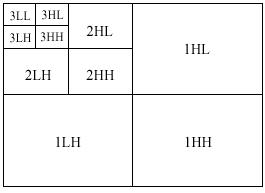
\includegraphics[width=0.3\textwidth, height=0.3\textwidth]{3stage_1}
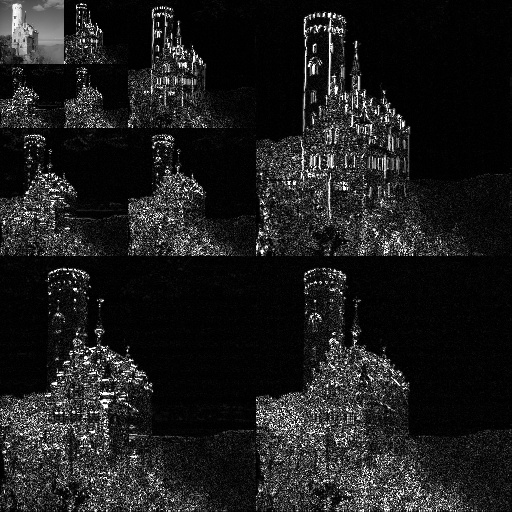
\includegraphics[width=0.3\textwidth]{3stage_2}
\caption[12pt]{3 Stage DWT \cite{jpeg2koverview}} \label{tab:title} 
\end{center}
\end{figure}
\subsubsection{Quantization}
Quantization is one necessary process for lossy compression. JPEG2000 was designed for lossless compression at beginning, but added lossy compression support after. In my project, I concentrate on near lossless compression of JPEG family, which need this quantization stage of compression processing. Quantization basically designed to reduce distinct value of given stream. When the number of discrete symbols in a given stream is reduces, the stream becomes more compressible. \\
In JPEG standard, after doing discrete cosine transform, we have a list of $8*8$ blocks. So JPEG's quantization will use a pre-defined quantization matrix to divide these blocks in order to have a bias but less complex blocks. \\
In JPEG2000, there isn't a pre-defined block size which means static quantization matrix is not exist. So I take an arbitry design to decrease entropy of image stream. Basically, two steps will be taken. First, after discrete wavelet transform, most items of results will be a float number rather than an integer.If we assume using static length coding, in most of systems, a float number need at least 4 bytes to store. After observing data, we can figure out that after 3 stage DWT, the biggest number of whole matrix is about 1500 and minimum number is about -20. So we just need at least 11 bits to store each item. If we assume using variety length coding, we can decrease about 1/3 of distinct values, which will provide approximately 4/7 deducation of coding length. So we need to first arbitry transform all data from float type to integers. Second, after taking round opertaion, we can find a lot of consederately small value in first stage's LH, HL, HH coeffiences. These small differences only show slightly different between two pixels of original image, but it takes more places to store them. Thus, we need the second step of quantization which is round more data close to 0. \\
\subsubsection{Coding}
JPEG2000 use arithmetic coder for low level coding operations. Embedded Block Coding with Optimal Truncation (EBCOT) is first step of coding. EBCOT is an implementation of compress by region of interests. It has some concepts of round to zero which has been covered in my quantization design. Basically, in this encoding process, each bit plane of the code block gets encoded in three so-called coding passes, first encoding bits (and signs) of insignificant coefficients with significant neighbors (i.e., with 1-bits in higher bit planes), then refinement bits of significant coefficients and finally coefficients without significant neighbors. The three passes are called Significance Propagation, Magnitude Refinement and Cleanup pass, respectively.\cite{jpeg2kwiki} After EBCOT, bits will be encoded by a context-driven binary arithmetic coder, namely the binary MQ-coder.
Unfortunately, MQ-coder and EBCOT are high computable uneffcience. In EBCOT, algorithm takes a great complexity. So, I didn't consider use EBCOT and MQ-coder as coding both in design and my own implementation. Instead of these techniques, I choose huffman coding, the one used in JPEG standard, as my coding system.
\subsection{JPEG-LS}


\section{Implementation}
In my project, I follow my design of section 3 to implement my work. To make my work content clearly, I draw everything on the process in Figure 2.
\begin{figure}[htb]
\begin{center}
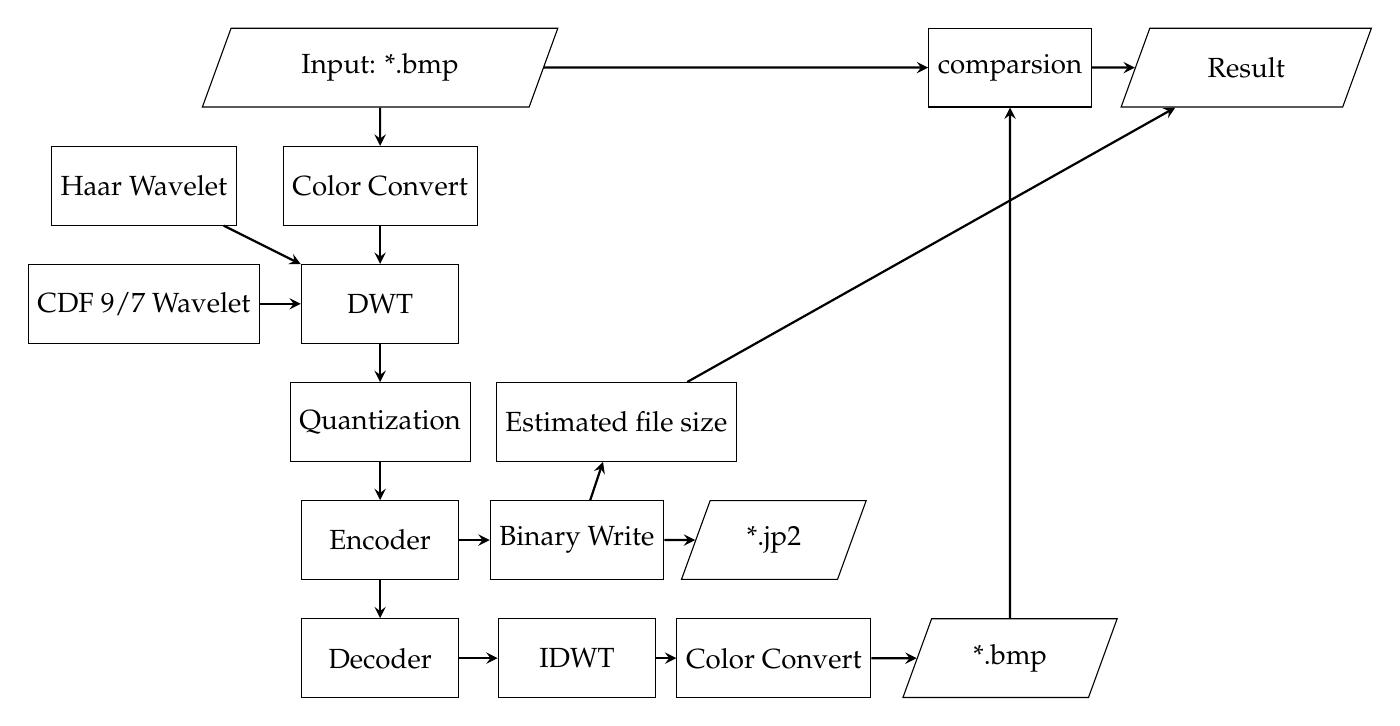
\begin{tikzpicture}[node distance=1.5cm, remember picture]
\tikzstyle{startstop} = [rectangle, rounded corners, minimum width=2cm, minimum height=1cm,text centered, draw=black]
\tikzstyle{io} = [trapezium, trapezium left angle=70, trapezium right angle=110, minimum width=2cm, minimum height=1cm, text centered, draw=black]
\tikzstyle{process} = [rectangle, minimum width=2cm, minimum height=1cm, text centered, draw=black]
\tikzstyle{decision} = [diamond, minimum width=2cm, minimum height=1cm, text centered, draw=black]
\tikzstyle{arrow} = [thick,->,>=stealth]
 %定义流程图具体形状
\node (input) [io] {Input: *.bmp};
\node (cvt) [process, below of=input] {Color Convert};
\node (dwt) [process, below of=cvt] {DWT};
\node (qua) [process, below of=dwt] {Quantization};
\node (enc) [process, below of=qua] {Encoder};
\node (bin) [process, right of=enc, xshift=1cm] {Binary Write};
\node (jp2) [io, right of=bin, xshift=1cm] {*.jp2};
\node (dec) [process, below of=enc] {Decoder};
\node (idwt) [process, right of=dec, xshift=1cm] {IDWT};
\node (icvt) [process, right of=idwt, xshift=1cm] {Color Convert};
\node (bmp) [io, right of=icvt, xshift=1.5cm] {*.bmp};
\node (cmp) [process, right of=input, xshift=6.5cm] {comparsion};
\node (res) [io, right of=cmp, xshift=1.5cm] {Result};
\node (haar) [process, left of=dwt, xshift=-1.5cm, yshift=1.5cm] {Haar Wavelet};
\node (cdf) [process, left of=dwt, xshift=-1.5cm] {CDF 9/7 Wavelet};
\node (size) [process, below of=bin,xshift=0.5cm, yshift=3cm] {Estimated file size};


 %连接具体形状
\draw [arrow](input) -- (cvt);
\draw [arrow](cvt) -- (dwt);
\draw [arrow](dwt) -- (qua);
\draw [arrow](qua) -- (enc);
\draw [arrow](enc) -- (bin);
\draw [arrow](bin) -- (jp2);
\draw [arrow](enc) -- (dec);
\draw [arrow](dec) -- (idwt);
\draw [arrow](idwt) -- (icvt);
\draw [arrow](icvt) -- (bmp);
\draw [arrow](input) -- (cmp);
\draw [arrow](bmp) -- (cmp);
\draw [arrow](cmp) -- (res);
\draw [arrow](haar) -- (dwt);
\draw [arrow](cdf) -- (dwt);
\draw [arrow](bin) -- (size);
\draw [arrow](size) -- (res);
\end{tikzpicture}
\caption[12pt]{Process of JPEG2000 Implementation} \label{tab:title} 
\end{center}
\end{figure}
Exactly as figure 2 shows, bmp files will be read into work process, first transformed to a YUV color domain. For Y, U, V channels, it applies wavelet transform to each of them. After quantization and encoding, estimated file size can be output and image will be write into a jp2 format file. Then, after decoding, inverse wavelet transform and inverse color coversion, program will output a bmp file. Then comparsion utlity will judge differential of original and target bmp file to infrustrate percentage of error.
\subsection{Haar Wavelet Transform}
My implementation of haar wavelet transform is very simple. For each stage, program will judge start and end pixel, and apply 2d DWT on target region.
\begin{spacing}{0.7}
\begin{algorithm}[htb]
\caption{2D Haar Discrete Cosine Transform}
   \begin{algorithmic}[1]
      \Function{Haar\_DWT}{$Matrix, height, width$}
        \For{$h = 0$ to $height$}
        		\For{$w = 0$ to $width$}
        			\State $Matrix[h][w] = sqrt(2) * (Matrix[h][w*2] + Matrix[h][w*2+1]) / 2$
        			\State $w = w + 2$
        		\EndFor
        		\State $h = h + 1$
        \EndFor
        \For{$w = 0$ to $width$}
        		\For{$h = 0$ to $height$}
        			\State $Matrix[h][w] = sqrt(2) * (Matrix[h*2][w] + Matrix[h*2+1][w]) / 2$
        			\State $h = h + 2$
        		\EndFor
        		\State $w = w + 1$
        \EndFor
       \EndFunction
       \\
      \Function{Haar\_DWT}{$Matrix, stage$}
      	\State $ h = Matrix.height$
      	\State $ w = Matrix.width$
        	\For{$ s = 0 $ to $ stage$}
        		\State $HAAR\_DWT( Matrix, h /pow(2,s), w/pow(2,s))$
        	\EndFor
      \EndFunction
\end{algorithmic}
\end{algorithm}
\end{spacing}
\subsection{CDF 9/7 Wavelet Transform}
CDF 9/7 is implementation by article "how does JPEG 2000 work?".\cite{jpeg2kwork} It turns that it doesn't work well even under very casual test experiments. Attaching my code below, which is mainly about transform, to prevent result bias, we also need to do some optimation in the end of this function, but that part is not such important, so I will discard it.
\begin{spacing}{0.7}
\begin{algorithm}[htb]
\caption{2D Haar Discrete Cosine Transform}
   \begin{algorithmic}[1]
   	  \State $ Array a = [-1.586, -0.053, 0.883, 0.444]$ \Comment{9/7 CDF Filter Coefficiences}
      \Function{Haar\_DWT}{$Matrix, height, width$}
        \For{$h = 0$ to $height$}
        		\For{$w = 0$ to $width-1$}
        			\State $Matrix[h][w] += a_1 * (Matrix[h][w-1] + Matrix[h][w+1])$
        			\State $w = w + 2$
        		\EndFor
        		\For{$w = 1$ to $width$}
        			\State $Matrix[h][w] += a_2 * (Matrix[h][w-1] + Matrix[h][w+1])$
        			\State $w = w + 2$
        		\EndFor
        		\For{$w = 0$ to $width-1$}
        			\State $Matrix[h][w] += a_3 * (Matrix[h][w-1] + Matrix[h][w+1])$
        			\State $w = w + 2$
        		\EndFor
        		\For{$w = 1$ to $width$}
        			\State $Matrix[h][w] += a_4 * (Matrix[h][w-1] + Matrix[h][w+1])$
        			\State $w = w + 2$
        		\EndFor
        		\State $h = h + 1$
        \EndFor
       \EndFunction    
\end{algorithmic}
\end{algorithm}
\end{spacing}
\subsection{Huffman Coding}
\subsection{File Organization}
\section{Comparsion}
\subsection{Metrics}
\subsection{Image Quality}
\begin{figure}[htbp]
\centering
\caption {PC Web Browser} \label{tab:title} 
\begin{tabular}{llr}
	\hline
	Operation & Comment & Traffic (KB)\\
	\hline
	Open Google Docs & & 1120.437\\
	\hline
	Open a document\footnotemark[1] & & 852.116\\
	\hline
	Do Nothing & & 0\\
	\hline
	Insert\footnotemark[2] at beginning & 1 character & 1.510\\
	 & 10 characters & 7.831 \\
	 & 100 characters & 76.231 \\
	 \hline
	 Insert at middle & 1 character & 3.070\\
	 & 10 characters & 7.858 \\
	 & 100 characters & 86.082 \\
	 \hline
	 Insert\footnotemark[3] at beginning & 100 characters & 6.204\\
	 \hline
	 Bold \& Unbold & bold &  39.409 \\
	 & unbold & 34.012 \\
	 \hline
	 Replace & replace "usa" to ")))", 125 occurrences & 96.745\\
	 & replace "op" to "]]", 802 occurrences & 645.305\\
	 \hline
	 Close a document & & 159.227\\
	 \hline
\end{tabular} 
\end{figure}
\footnotetext[2]{This document is about 1000 KB}
\subsection{Compression Ratio}


\section{Summary}


\section{Acknowledgement}


\section{Appendix A: How to run the software}





\begin{thebibliography}{9}
\bibitem{jpegcommiteewiki} 
Wikipedia: Joint Photographic Experts Group Wiki,\\
\texttt{https://en.wikipedia.org/wiki/Joint\_Photographic\_Experts\_Group}
\bibitem{jpegwiki} 
Wikipedia: JPEG Wiki,
\texttt{https://en.wikipedia.org/wiki/JPEG}
\bibitem{jpeg2kwiki} 
Wikipedia: JPEG 2000 Wiki,
\texttt{https://en.wikipedia.org/wiki/JPEG\_2000}
\bibitem{jpegls} 
JPEG: Overview of JPEG-LS,
\texttt{https://jpeg.org/jpegls/}
\bibitem{hwtmath} 
How Math Led to the JPEG2000 Standard:Haar Wavelet Transformation,\\
\texttt{http://www.whydomath.org/node/wavlets/hwt.html}
\bibitem{jpeg2koverview} 
C. Christopoulos, A. Skodras, and T. Ebrahimi.  “The JPEG2000 Still Image Coding: An Overview,” IEEE Transactions on Consumer Electronics, Vol. 46, No. 4, pp. 1103-1127, November 2000,\\
\texttt{http://etro.vub.ac.be/\~chchrist/paper\_ieee\_ce\_jpeg2000\_Nov2000.pdf}
\bibitem{jpeg2kwork} 
Prof. Edward Aboufadel.  “JPEG 2000: The Next Compression Standard using wavelet technology”,\\
\texttt{http://faculty.gvsu.edu/aboufade/web/wavelets/student\_work/EF/how-works.html}
\end{thebibliography}
\end{document}